\documentclass{beamer}

\usepackage[utf8]{inputenc}
\usepackage[ngerman]{babel}
\usepackage[T1]{fontenc}

\usepackage{amsmath,amssymb,amsfonts,amsthm,mathtools}

\usepackage{paralist}

%\usepackage[algoruled,algo2e,vlined,titlenotnumbered,german]{algorithm2e}
\usepackage{algorithm}
\usepackage{algorithmic}
\usepackage{tikz}

\mode<presentation>
{
  \setbeamertemplate{navigation symbols}{}
    \usetheme{Hannover}
   \setbeamercovered{transparent}
   \useoutertheme{infolines}
}


\title[Simulation normalisierter Prozesse] % (optional, nur bei langen Titeln noetig)
{Simulation normalisierter BPDL und TSS Prozesse}
\subtitle{2. Vortrag des Begleitseminars}
\author[B.Prochnau] % (optional, nur bei vielen Autoren)
{Boris Prochnau}
\institute[Universität Bonn]{Institut für Angewandte Mathematik\\Universität Bonn}

\date {\today}
\setbeamercovered{invisible}

\begin{document}
%
% ****************************************************************************************************
%					preliminaries
% ****************************************************************************************************
%

\begin{frame}
  \titlepage
\end{frame}
\begin{frame}
  \frametitle{Übersicht}
  \tableofcontents
\end{frame}

\section{Ziele}
	\begin{frame}
		\frametitle{Ziele der Bachelorarbeit}
		\begin{itemize}
			\item Simulation eines normalisierten BPDL Prozesses
			\item Simulation eines normalisierten TSS Prozesses
		\end{itemize}
	\end{frame}

\section{Model}
	\begin{frame}
		\frametitle{Grundlagen - Wiederholung}
		\begin{itemize}
			\item Jedes Individuum hat ein Merkmal $ x \in X $. \\
			Der Einfachheit halber sei X eine Indexmenge: $ X = \{1,\dots, n\} $ repräsentativ für eine Durchzählung der Merkmale.
			\pause
			\item Jedes Individuum kann sich asexuell fortpflanzen oder sterben
			\pause
			\item Diese Ereignisse sind exponentiell verteilte Zeitpunkte. 
		\end{itemize}		
	\end{frame}
	\begin{frame}
		\frametitle{Raten}
		Mit folgenden Raten:
		\begin{itemize}
			\item b(x): Geburtenraten durch ein Individuum mit Merkmal x
			\pause
			\item d(x): natürliche Todesrate
			\pause
			\item c(x,y): Todesrate durch Wettbewerb zwischen Individuen mit Merkmal x und y.
			\pause
			\item $ \mu $: Mutationswahrscheinlichkeit "{}auf die Nachbarn"{} mit je $ \frac{\mu}{2} $ pro Nachbar. 
		\end{itemize}
	\end{frame}
	\begin{frame}
		\frametitle{kompakte Raten - Superposition}
		Zusammenfassen der Ereignisse ergibt:
		\begin{itemize}
			\item intrinsische Geburtenrate: $ b(x) \cdot (1 - \mu) $
			\pause
		 	\item Todesrate: $ d(x) + \sum_{i=1}^{N_t} c(x,x_i) $, $ N_t = \#Individuen$ zum Zeitpunkt t, und \underline{$ x_i $ das Merkmal des i-ten Individuums}.
		 	\pause
		 	\item ODER Todesrate: $ d(x) + \sum_{i=1}^{n} c(x,x_i) \cdot n_t(x_i) $, $ n = \#Merkmale$, und $ n_t(x_i) = \#Individuen $ mit \underline{Merkmal $ x_i $} zur Zeit t.
		\end{itemize}
	\end{frame}	
	\begin{frame}
		\frametitle{Merkmale im Blickpunkt}
		Programm soll Entwicklung der Merkmale simulieren, nicht der Individuen:
		\pause
		\begin{itemize}
			\item Geburtenrate (Wachstumsrate) des Merkmals x: 
			\begin{align*}
				B(x) & = b(x) \cdot (1 - \mu) \cdot n_t(x) \\
				& + \frac{\mu}{2} \cdot b(x+1)\cdot n_t(x+1) \\ 
				& + \frac{\mu}{2} \cdot b(x-1)\cdot n_t(x-1)
			\end{align*}
			\pause
			\item Todesrate des Merkmals x: 
			\[ D(x) = d(x) \cdot n_t(x) + n_t(x) \cdot \sum_{i=1}^{n} c(x,x_i) \cdot n_t(x_i) \]
		\end{itemize}
		\pause
		$ \Rightarrow $ 2 exponentiellen Uhren (Zeitpunkten) pro Merkmal
	\end{frame}	
	\begin{frame}
		\frametitle{Totale Ereignis Rate}
		Zusammenfassung zu einer Uhr pro Evolutionssprung:
		\pause
		\begin{itemize}
			\item Ereignisrate des Merkmals x (Trait Rate):
				\[ TR(x) = B(x) + D(x) \]
			\item Totale Ereignis Rate (Total Event Rate): 
			\[ TER = \sum_{x \in X} TR(x)\]
		\end{itemize}
		Die TER entspricht einer Rate für das erste klingeln der Merkmale.
	\end{frame}
	\begin{frame}
		\frametitle{Population als Zufallsvariable - Wiederholung}
		\pause
		Die Population ist ein Markov Sprungprozess der durch Zufallsvariablen
		\[ \nu_t = \sum_{i=1}^{N_t} \delta_{x_i}, \text{ mit } \int_X 1\nu_t(dx) = N_t \]
		beschrieben wird.\\
		Wobei:
		\[ \nu_t \in M_F(X) = \left\{ \sum_{i=1}^{n} \delta_{x_i}, n \in \mathbb{N}, x_1, \dots, x_n \in X \right\} \]
	\end{frame}
	
	
	\subsection{Normalisierung}
		\begin{frame}
			\frametitle{Large Population Approximation}
			Die LPA Normalisierung erweitert die Betrachtung auf die Ebene der Population. 
			\pause
			Dafür wird der Prozess mit einem Parameter K skaliert:
			\[ \nu_t^K := \frac{1}{K} \nu_t \]
			\pause
			Mit Anpassungen:
			\begin{itemize}
				\item $ n_0^K $ wird proportional zu K gewählt
				\pause
				\item Raten für Geburten und natürliche Tode der Individuen bleiben unverändert
				\pause
				\item Jedoch: $ c^K = \frac{c}{K} $
				\pause
				\item proportionale Anpassung von $ \mu $
			\end{itemize}
		\end{frame}
		\begin{frame}
			\frametitle{Beispiel: K= 100}
			\begin{figure}[H]
				\centering
				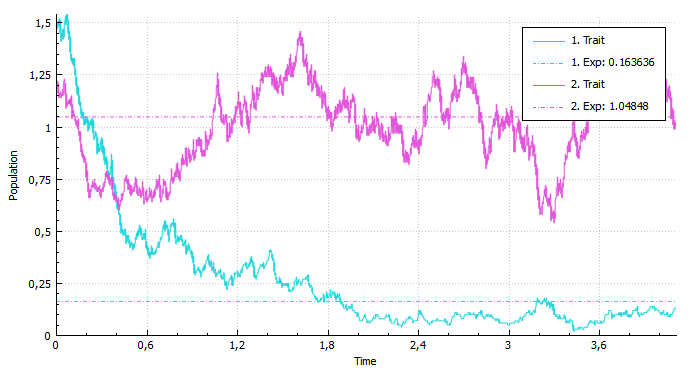
\includegraphics[width=1\linewidth]{./LPANormalisierungK100}
				\caption[LPAK100]{LPA Normalisierung mit K=100}
				\label{LPA Normalisierung K=100}
			\end{figure}
		\end{frame}
		\begin{frame}
			\frametitle{Beispiel: K= 10000}
			\begin{figure}[H]
				\centering
				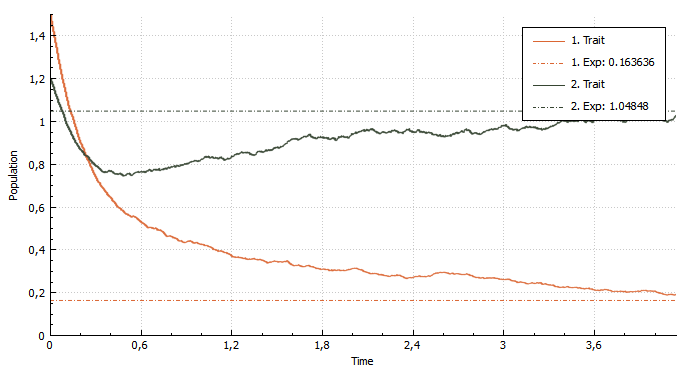
\includegraphics[width=1\linewidth]{./LPANormalisierungK10000}
				\caption[LPAK100]{LPA Normalisierung mit K=10000}
				\label{LPA Normalisierung K=10000}
			\end{figure}
		\end{frame}
		
	\subsection{Equilibrium}
		\begin{frame}
			\frametitle{stabile Zustände}
			Im stabilen Zustand ändert sich die Populationsgröße nicht mehr:
			\pause
			\begin{itemize}
				\item Für Monomorphe Population:
					\begin{align*}
					0 & = \dot{n} = (b(x) - d(x) - \bar{n}c(x,x))\bar{n}\\
					\bar{n}_x &= \frac{\left[ b(x)-d(x) \right]_+}{c(x,x)}
					\end{align*}
					\pause
				\item Für Dimorphe Population:
					\[ n_x = \frac{(b(x) - d(x))c(y,y)-(b(y)-d(y))c(x,y)}{c(y,y)c(x,x) - c(y,x)c(x,y)} \]
					oder $ (\bar{n}_x, 0)$, $ (0, \bar{n}_y)$ bzw. $ (0,0) $
			\end{itemize}
		\end{frame}
\section{Algorithmus}
	\begin{frame}
		\frametitle{Evoultion Step}
		Der Simulation liegt ein Algorithmus zugrunde der einen Sprung des Markov Sprung Prozesses durchführt.
		\pause
			\begin{algorithm}[H]
				\caption{EvolutionStep()}
				\begin{algorithmic}[1]
					\ENSURE{A full evolution Step happened}
					\STATE calculateEventRates();
					\STATE sampleEventTime();
					\STATE changeATrait();
				\end{algorithmic}
			\end{algorithm}
	\end{frame}
	\begin{frame}
		\frametitle{Evoultion Step - detailierter}
		Von dieser werden folgende Berechnungen angestoßen:
		\pause
			\begin{algorithm}[H]
				\caption{EvolutionStep()}
				\begin{algorithmic}[1]
					\ENSURE{A full evolution Step happened}
					\STATE ---$>$calculateEventRates();
					\STATE calculateTotalDeathRates()
					\STATE calculateTotalBirthRates()
					\STATE calculateTotalEventRate()
					\STATE ---$>$sampleEventTime();
					\STATE sampleEventTime();
					\STATE ---$>$changeATrait();
					\STATE choseTraitToChange();
					\STATE choseEventType();
					\STATE executeEventTypeOnTrait();
				\end{algorithmic}
			\end{algorithm}
	\end{frame}
	
\section{Simulation}
	\subsection{Aufgabenteilung und Flexibilität}
		\begin{frame}
			\frametitle{Flexibilität}
			Um Flexibilität aufrecht zu erhalten werden die Arbeitsbereiche im Code getrennt gehalten\\
			\pause
			Grund der Idee:
			\begin{itemize}
				\item Möglichst viel Unabhängigkeit
				\pause
				\item verhindert "Coderot" - faulen Code
				\pause
				\item steigende Komplexität führt nicht zu undefiniertem Verhalten
				\pause
				\item "{}Single Responsibility Principle"{}
				\pause
				\item Keine Klassen die zu viel Wissen
			\end{itemize}
		\end{frame}
		\begin{frame}
			\frametitle{Arbeitsmodule}
			Die Architektur besteht aus 3 Modulen
			\pause
			\begin{figure}[H]
				\centering
				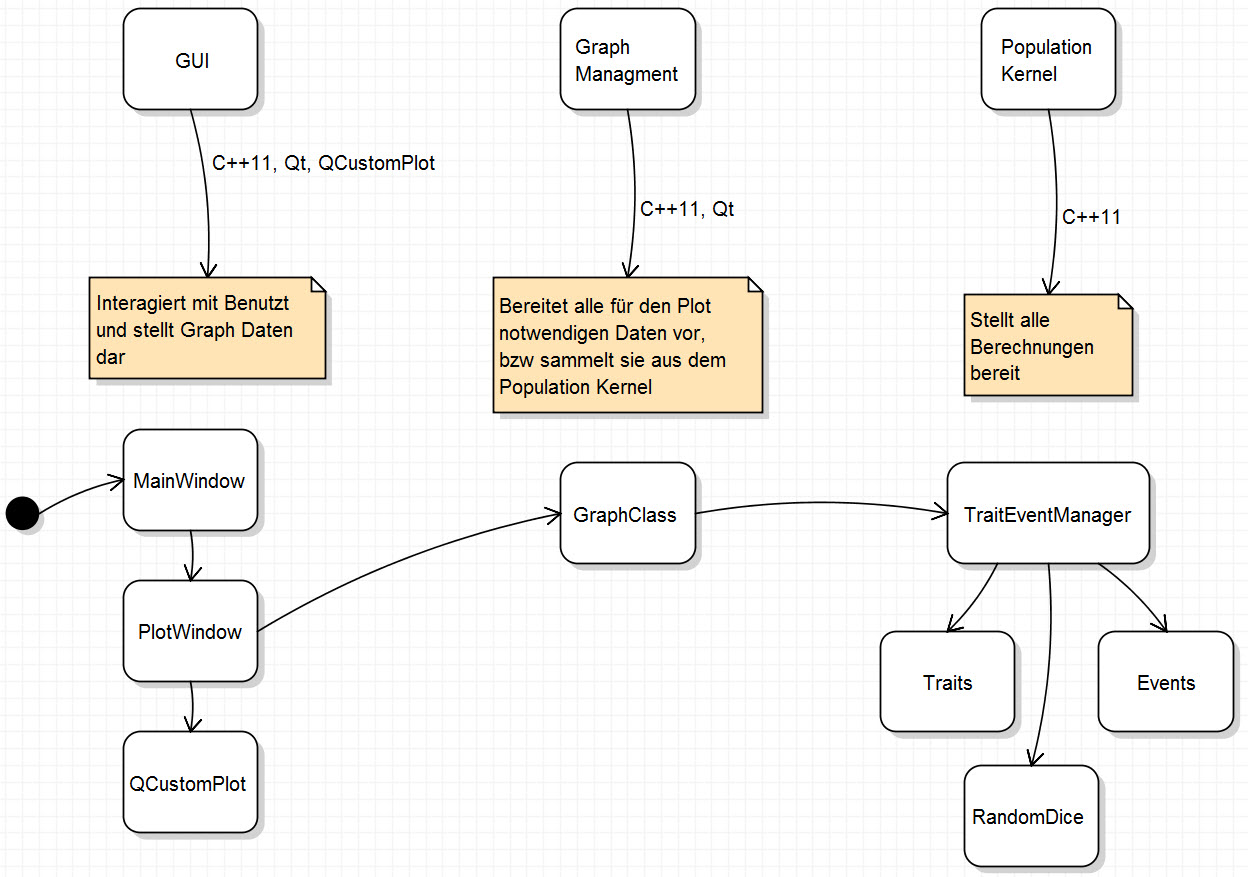
\includegraphics[width=0.8\linewidth]{./Bild_Module}
				\caption[Module]{Arbeitsmodule und Klassenabhängigkeiten}
				\label{Module und Klassen}
			\end{figure}
		\end{frame}
	\subsection{Layout}
		\begin{frame}
			\frametitle{Layout: Lesen der Parameter}
			Parameter sollten aus \underline{Dateien} gelesen werden können:
			\pause
			\begin{figure}[H]
				\centering
				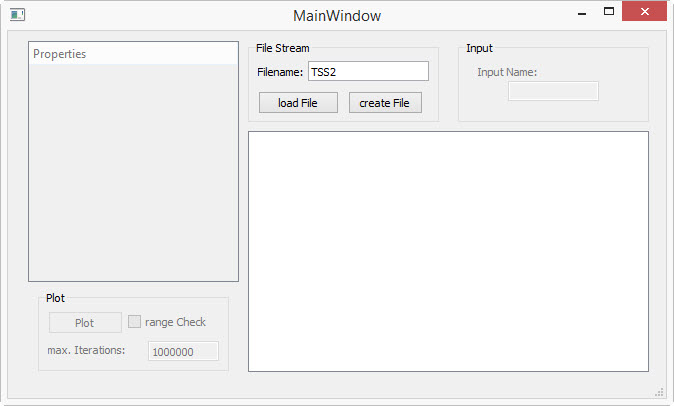
\includegraphics[width=0.9\linewidth]{./MainWindow_Start}
				\caption[Startwindow]{MainWindow nach dem Start}
				\label{MainWindow_Start}
			\end{figure}
		\end{frame}
		\begin{frame}
			\frametitle{Anzeige der Parameter}
			Baumdarstellung der Parameter:
			\pause
			\begin{figure}[H]
				\centering
				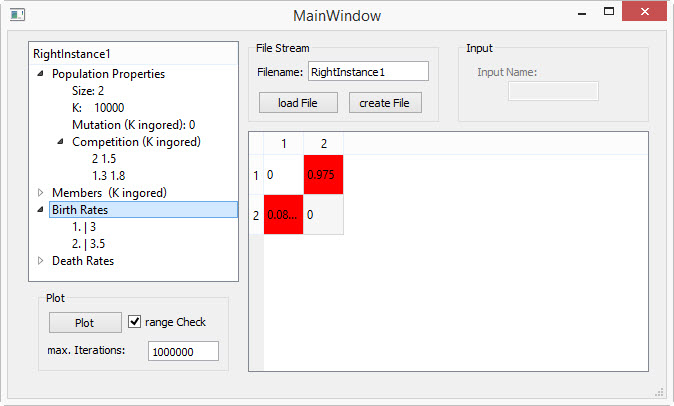
\includegraphics[width=0.9\linewidth]{./MainWindow_ParameterBaum}
				\caption[MainWindow_Parameter]{MainWindow mit geladenen Parametern}
				\label{Baumstruktur}
			\end{figure}
		\end{frame}
		\begin{frame}
			\frametitle{Erstellen neuer Testinstanzen}
			Anlegen einer neuen Datei:
			\pause
			\begin{figure}[H]
				\centering
				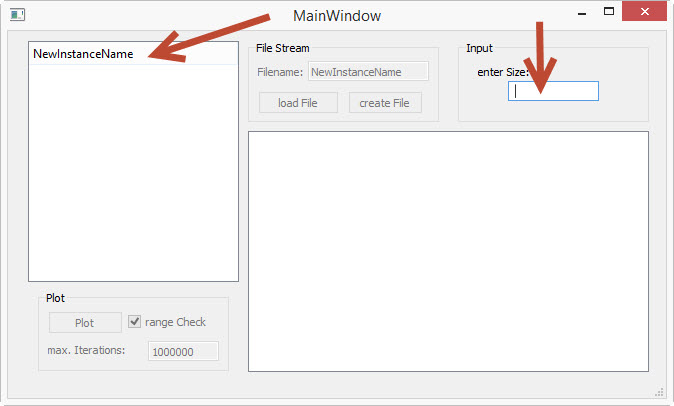
\includegraphics[width=0.8\linewidth]{./MainWindow_createFile}
				\caption[erstelle Datei]{Nach Klick auf "create File" werden die neuen Parameter einzeln abgefragt}
				\label{fig:MainWindow_createFile}
			\end{figure}
		\end{frame}
		\begin{frame}
			\frametitle{Testinstanz erstellt}
			\begin{figure}[H]
				\centering
				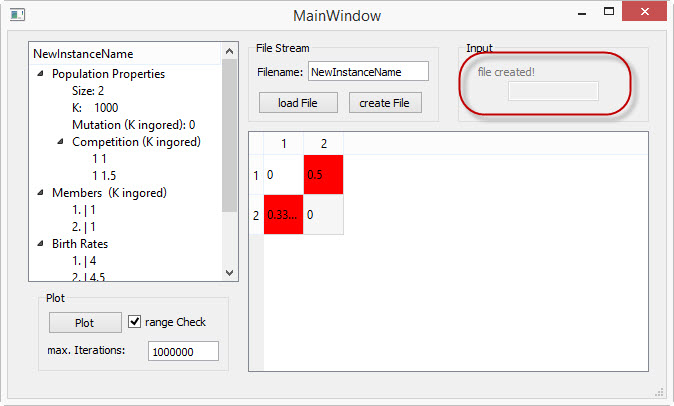
\includegraphics[width=1\linewidth]{./MainWindow_FileCreated}
				\caption[Datei erstellt]{Nach eingabe des letzten Parameters}
				\label{fig:MainWindow_FileCreated}
			\end{figure}
		\end{frame}
		\begin{frame}
			\frametitle{Darstellung der Graphen}
			Was soll die graphische Darstellung der Graphen erfüllen?
			\pause
			\begin{itemize}
				\item Anzeige des simulierten Prozesses
				\pause
				\item Zoom und Bewegung auf einem Koordinatensystem
				\pause
				\item Abspeichern aktueller Bilder für spätere Vergleiche
				\pause
				\item Verhindern dass die Berechnung das Programm einfriert
			\end{itemize}
		\end{frame}
		\begin{frame}
			\frametitle{Start der Darstellung}
			Nach dem drücken des "{}Plot"{} Buttons öffnet sich ein Fenster
			\pause
			\begin{figure}[H]
				\centering
				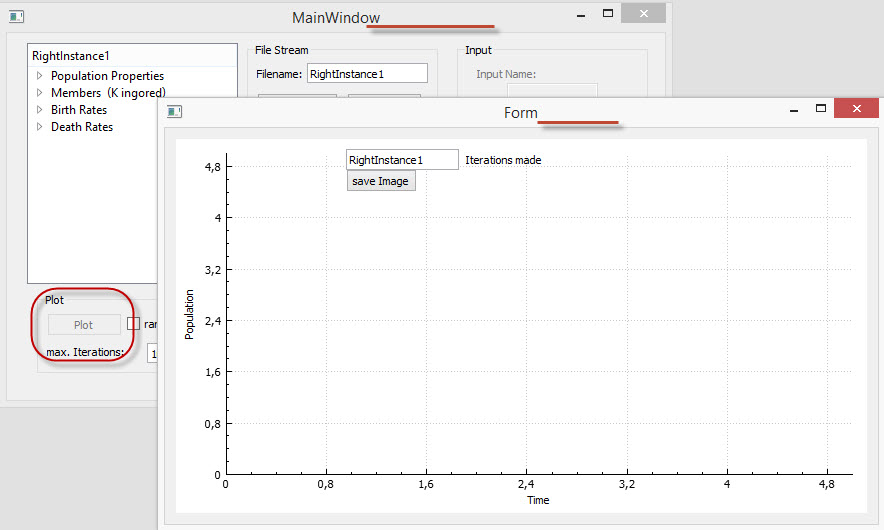
\includegraphics[width=0.8\linewidth]{./PlotWindow_start}
				\caption[PlotWindow_start]{Start des PlotWindow}
				\label{PlotWindow_start}
			\end{figure}
		\end{frame}
		\begin{frame}
			\frametitle{Arbeit im Hintergrund}
			Was fällt auf?
			\begin{itemize}
				\item Der Plot Button kann nicht mehr betätigt werden. Das verdeutlicht, dass der Prozess gerade simuliert wird
				\pause
				\item Trotz der Berechnungen friert das Bild nicht ein und verursacht keinen Konflikt mit der Betriebssystem-Sicherheit:
				\pause
				\begin{figure}[H]
					\centering
					
\includegraphics[width=0.6\linewidth]{./KeineRueckmeldungSmall}
					\caption[Keine Rueckmeldung]{Bsp: Überlasteter Hauptthread}
					\label{Keine Rueckmeldung}
				\end{figure}
			\end{itemize}
		\end{frame}
		\begin{frame}
			\frametitle{Darstellung der Graphen}
			Wenn ein günstiger Zustand erreicht wurde, oder maximal viele Iterationen gemacht wurden, werden die Punkte verbunden:
			\pause
			\begin{figure}[H]
				\centering
				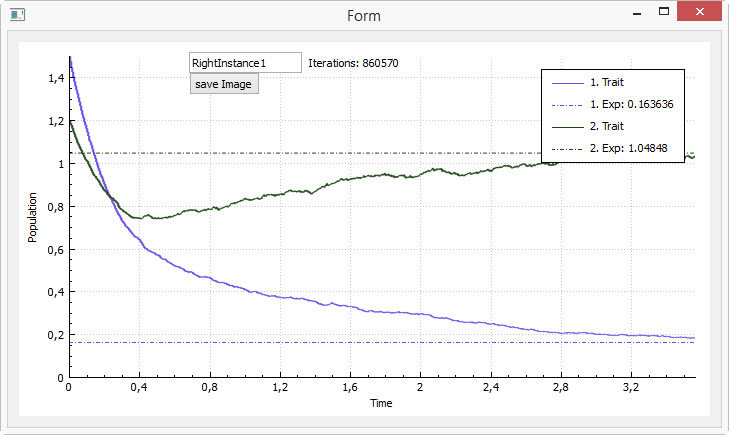
\includegraphics[width=0.7\linewidth]{./PlotWindow_smallBPDL}
				\caption[PlotWindow]{PlotWindow mit Dimorpher Population}
				\label{PlotWindow}
			\end{figure}
		\end{frame}
		\begin{frame}
			\frametitle{Was wurde Dargestellt?}
			\pause
			\begin{itemize}
				\item Die Entwicklung der beiden Merkmale mit Zeit und Größe
				\item Die stabilen Zustände (gestrichelt)
				\item Die Anzahl der tatsächlich gemachten Sprünge
				\item Einen Button zum Speichern des Bildes
				\item Eine Legende die jeden Graphen beschreibt
			\end{itemize}
		\end{frame}
		\begin{frame}
			\frametitle{Zoom und Bewegungsfreiheit}
			Zoom, Bewegungsfreiheit und Reskalierung des Plots sind auch möglich:
			\begin{figure}[H]
				\centering
				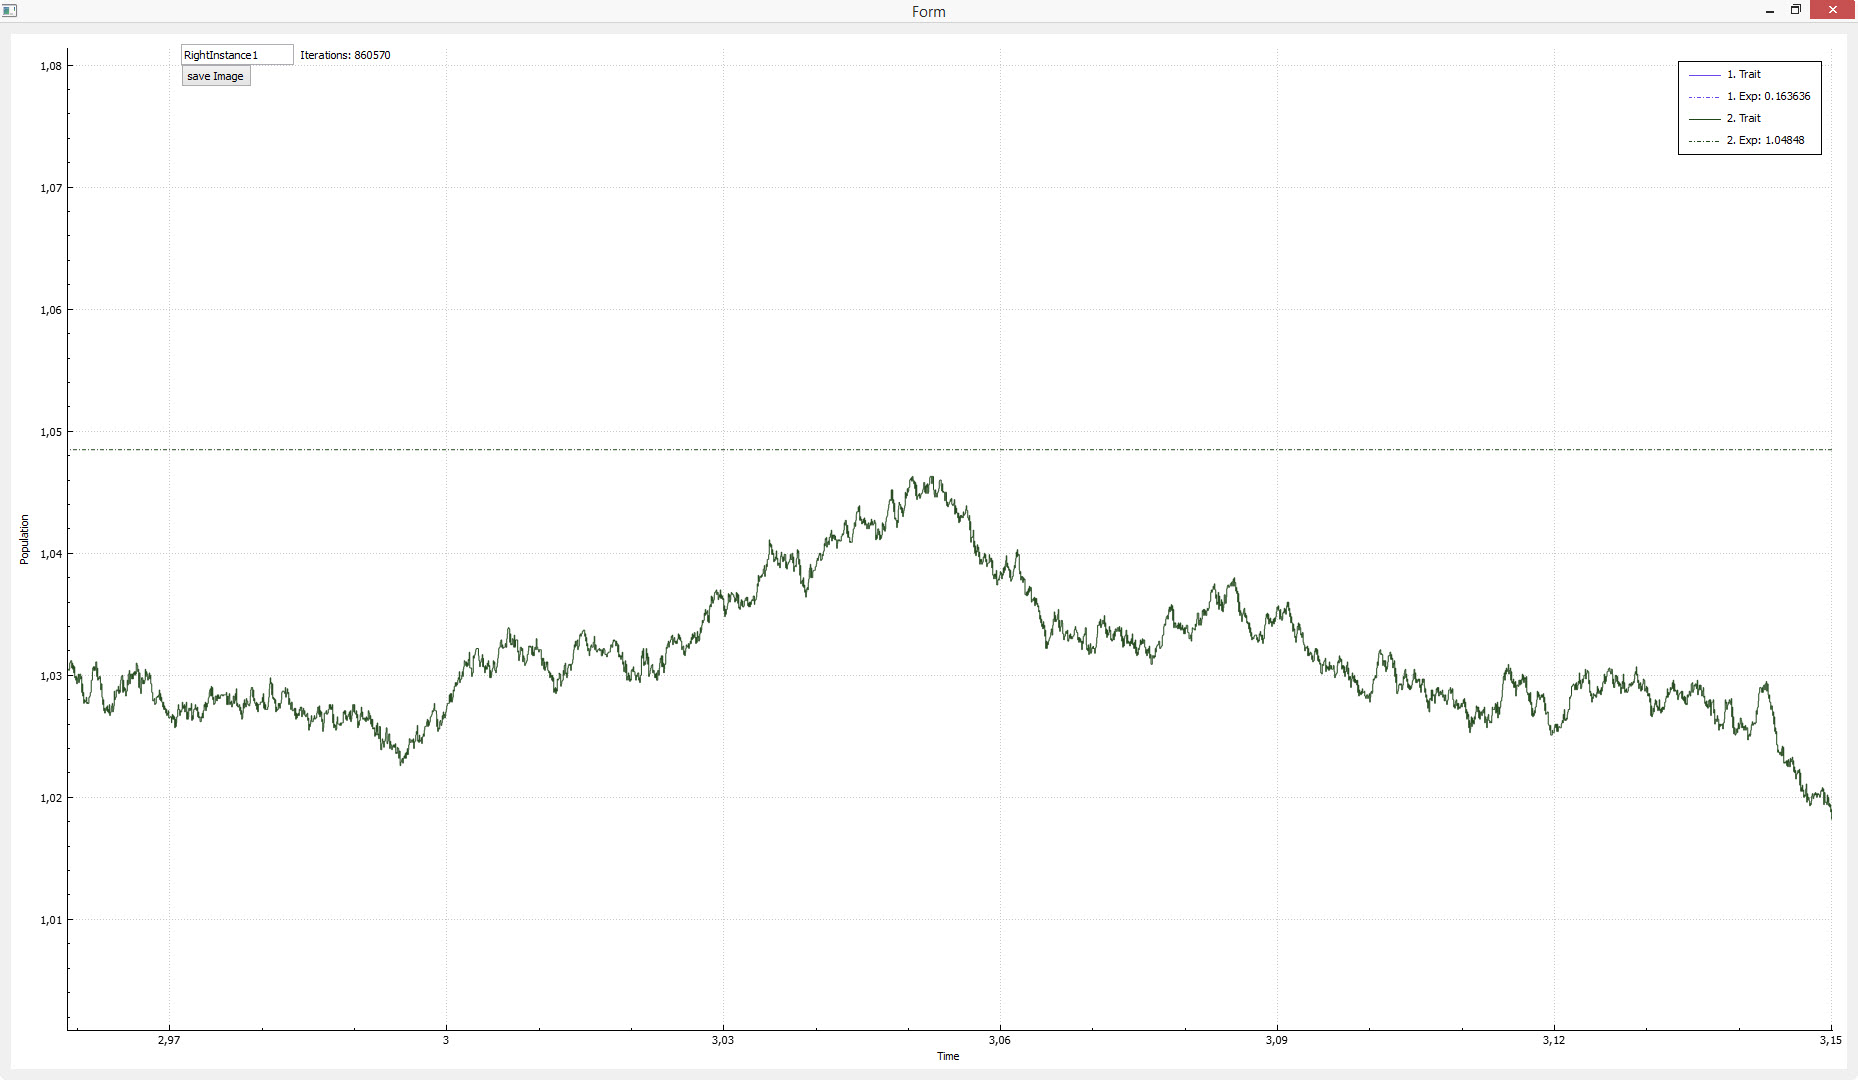
\includegraphics[width=0.8\linewidth]{./PlotWindow_zoomedBPDL}
				\caption[ZoomBPDL]{Plot wurde maximiert, gezoomt und bewegt}
				\label{fig:PlotWindow_zoomedBPDL}
			\end{figure}
		\end{frame}

\section{Korrektheit der Implementation}
	\begin{frame}
		\frametitle{Korrektheit: Testgetriebenen Entwicklung}
		\pause
		\begin{itemize}
			\item Die Korrektheit der Implementation ist mit zunehmender Komplexität des Codes schwerer zu prüfen (besonders bei Zufallsbedingten Simulationen)
			\pause
			\item Zu diesem Zweck verwende ich das Prinzip der "Testgetriebenen Entwicklung" (Test Driven Development)
			\pause
			\item Dabei werden Funktionen mit erwartetem Verhalten verglichen
		\end{itemize}
		\pause
		Folgend ein Beispiel:
	\end{frame}
	\begin{frame}
		\frametitle{Einfaches Testbeispiel}
		\begin{figure}[H]
			\centering
			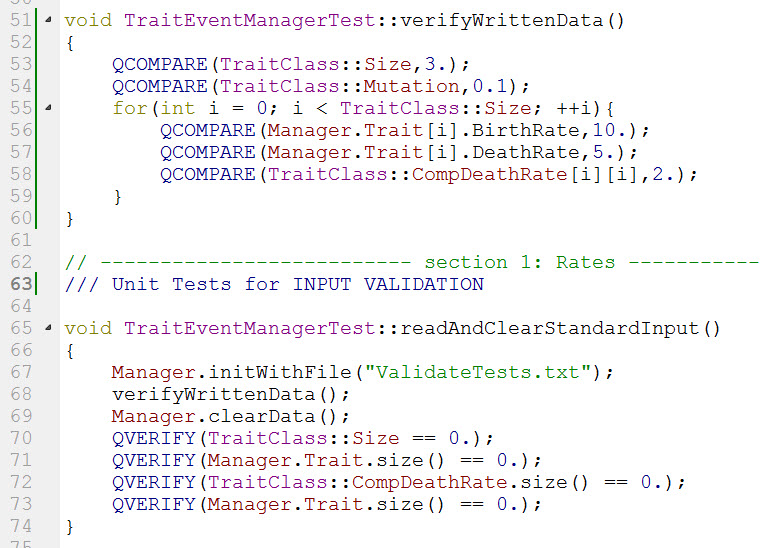
\includegraphics[width=0.85\linewidth]{./UnitTest}
			\caption[UnitTest]{Unit Test versichert korrektes lesen aus Datei}
			\label{Unit Test}
		\end{figure}
	\end{frame}
	\begin{frame}
		\frametitle{Testdurchlauf}
		Der Output einer Testsammlung kann so beginnen:
		\pause
		\begin{figure}[H]
			\centering
			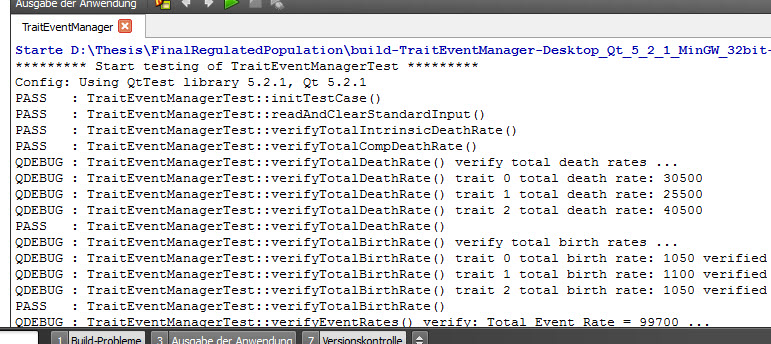
\includegraphics[width=0.9\linewidth]{./TestResult_start}
			\caption[Test Resultat einer Test Datei]{Ergebnisse einiger Tests}
			\label{Test Results}
		\end{figure}
		\pause
		Tests ermöglichen zusätzlich komplexere Simulationen
	\end{frame}

\section{TSS - Prozesse}
	\begin{frame}
		\frametitle{Trait Substitution Sequence}
		\begin{itemize}
			\item Wie bei LPA-Normalisierung ergeben sich TSS-Prozesse als Grenzprozesse von BPDL-Prozessen
			\item Jedoch mit wachsendem K schrumpft $ \mu $ mit der Ordnung:
			\[ \frac{1}{e^{VK}} << \mu_K << \frac{1}{K log(K)} \]
			\item Weiterhin wird die Zeit skaliert so dass die Verdrängungszeit infinitesimal klein wird
			\item Für die Simulation bedeutet es, dass sehr viele Sprünge um das Equilibrium zu erwarten sind
		\end{itemize}
	\end{frame}
	\begin{frame}
		\frametitle{Bisheriger Simulationsstand}
		Eine Simulation würde bisher so aussehen (K = 1000):
		\pause
		\begin{figure}[H]
			\centering
			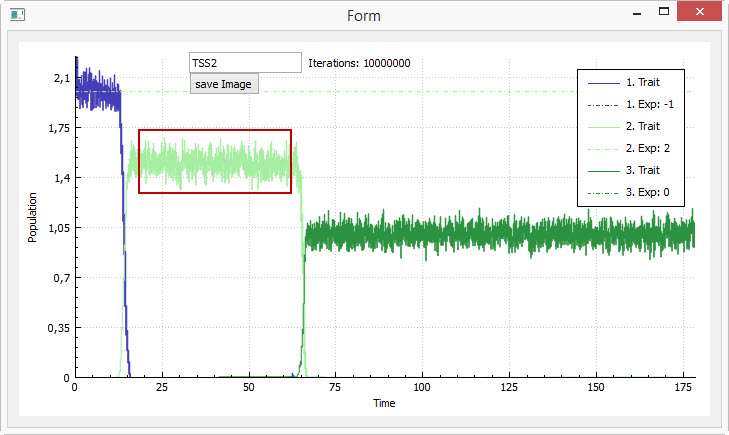
\includegraphics[width=0.8\linewidth]{./TSS_BPDLSimulation}
			\caption[TSS Prozess]{TSS Prozess mit K=1000}
			\label{fig:TSS_BPDLSimulation}
		\end{figure}

	\end{frame}
	
	\subsection{Fitness}
		\begin{frame}
			\frametitle{Fitness-Funktion}
			\pause
			\[ f(x,y) = b(x) - d(x) - c(x,y)\bar{n}_y \]
			\pause
			\begin{itemize}
				\item Sie gibt an wie gut sich ein Merkmal durchsetzten kann
				\item Asymptotische Wachstumsrate von y, wenn x im Zustand $ \bar{n}_x $ ist und y nur wenige Individuen hat
				\item Ermöglicht Aussagen über die Überlebenswahrscheinlichkeit einer Mutation
				\item Ermöglicht Aussagen über die angenommenen stabilen Zustände.
			\end{itemize}
			\pause
			Da wir nur eine Mutation zu den Nachbarn berücksichtigen, ist unsere Fitness Matrix eine Bandmatrix
		\end{frame}
		\begin{frame}
			\frametitle{Fitness-Matrix}
			Fitness-Matrix wird sofort beim Laden der Parameter berechnet und angezeigt:
			\begin{figure}[H]
				\centering
				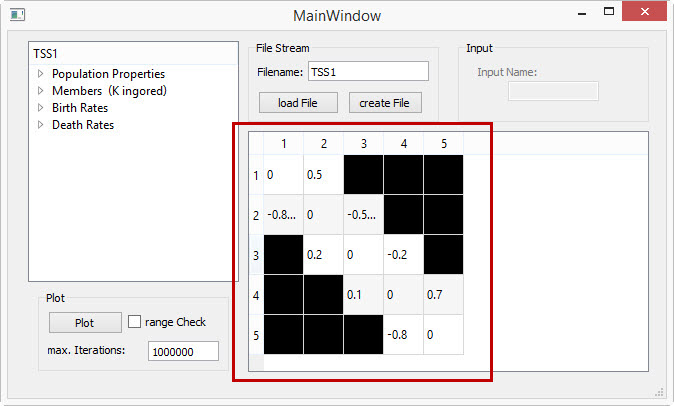
\includegraphics[width=0.7\linewidth]{./MainWindow_BandMatrix}
				\caption[Fitness Matrix]{Fitness Bandmatrix}
				\label{MainWindow mit Fitness Bandmatrix}
			\end{figure}
		\end{frame}
		\begin{frame}
			\frametitle{Eigenschaften der Fitness}
			Was erwartet die Simulation von der Fitness?\\
			\pause
			Im dimorphen Fall gilt:
			\begin{itemize}
				\item $ f(y,x) < 0 \Rightarrow (\bar{n}_x,0) $ ist ein stabiler Zustand
				\item $ f(y,x) > 0 \wedge f(x,y) < 0 \Rightarrow (\bar{n}_x,0) $ ist ein stabiler Zustand
			\end{itemize}
			\pause
			Für TSS-Prozesse gilt:
			\begin{itemize}
				\item $ f(y,x) > 0 \wedge f(x,y) < 0 $, x wird durch y verdrängt
				\item $ f(y,x) > 0 \wedge f(x,y) > 0 $, Koexistenz
			\end{itemize}
		\end{frame}	
		\begin{frame}
			\frametitle{Invasion}
			\pause
			Die Fitness ermöglicht eine Grenzwertaussage über die Invasionswahrscheinlichkeit:
			\[ \frac{\left[ f(y,x)\right]_+ }{b(y)} \]
			\pause
			Mit diesen Informationen lässt sich die Anzeige der Fitnessmatrix mit mehr Optionen ausstatten:\\
			\pause
			Einträge werden:
			\begin{itemize}
				\item Rot - falls eine Koexistenz von Merkmalen zu erwarten ist 
				\item Grün - falls die Invasionswahrscheinlichkeit hoch ist
			\end{itemize}
			Geplant ist eine stufenweiser Anstieg von hellem zu dunklem Grün. Wurde noch nicht implementiert.
		\end{frame}	
		\begin{frame}
			\frametitle{Fitnessmatrix mit farblichen Akzenten}
			Hier sieht man eine Fitnessmatrix mit grünen und roten Einträgen. Dabei wird ein Eintrag grün wenn er eine Invasionswahrscheinlichkeit von mindestens 50\% aufweist.
			\begin{figure}[H]
				\centering
				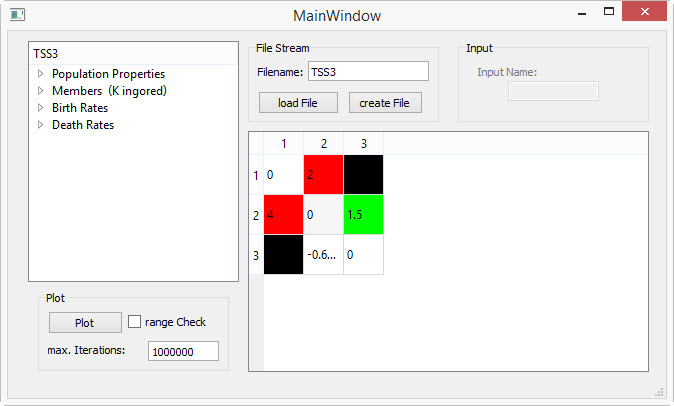
\includegraphics[width=0.7\linewidth]{./MainWindow_red_green_loaded}
				\caption[MainWindow_redGreenFitness]{Fitness Matrix mit roten und gruenen akzenten}
				\label{fig:MainWindow_red_green_loaded}
			\end{figure}
		\end{frame}	
		
	\subsection{Interpolation}
		\begin{frame}
			\frametitle{Optimierung}
			Um die Simulationsdauer zu reduzieren würde sich eine lineare Interpolation des Prozesses anbieten. Die rechnerische Entlastung wird im folgenden Bild deutlich dargestellt:
			\pause
			\begin{figure}[H]
				\centering
				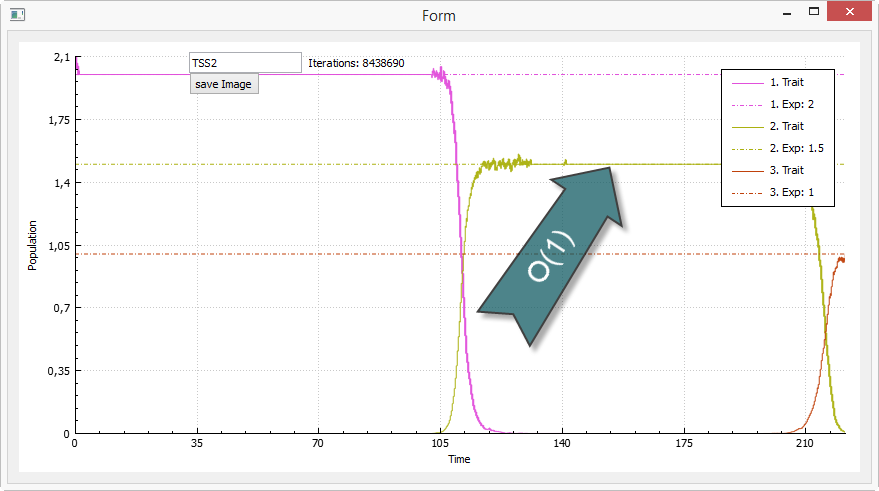
\includegraphics[width=0.7\linewidth]{./TSS_interpolated}
				\caption[TSS_interpolated]{TSS Prozess für K = 10000}
				\label{fig:TSS_interpolated}
			\end{figure}
		\end{frame}	
		\begin{frame}
			\frametitle{Optimierung}
			Außerdem verbessert sich damit die Lesbarkeit. Damit ist es möglich die Mutationspunkte und deren Auswirkungen genauer zu studieren:
			\pause
			\begin{figure}[H]
				\centering
				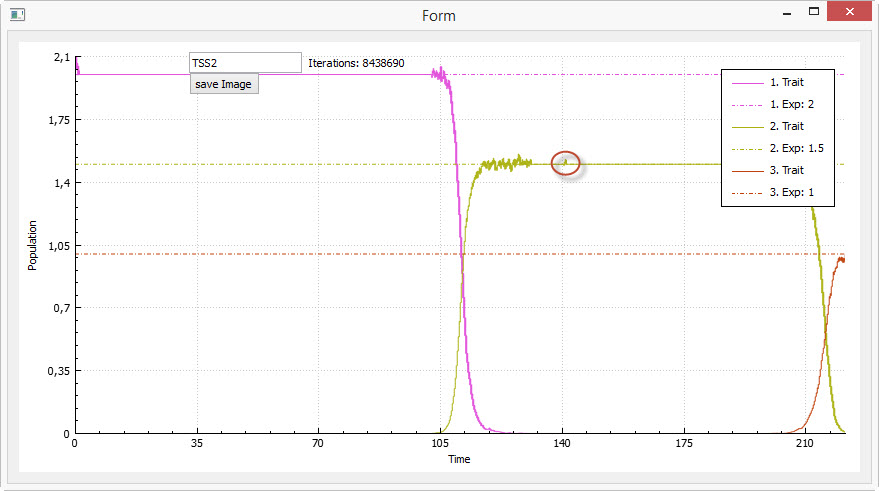
\includegraphics[width=0.8\linewidth]{./TSS_Mutation}
				\caption[Invasionsversuch]{Invasionsversuch deutlich zu erkennen}
				\label{fig:TSS_Mutation}
			\end{figure}
		\end{frame}	
		\begin{frame}
			\frametitle{Optimierung}
			Näher betrachtete Auswirkungen:
			\pause
			\begin{figure}[H]
				\centering
				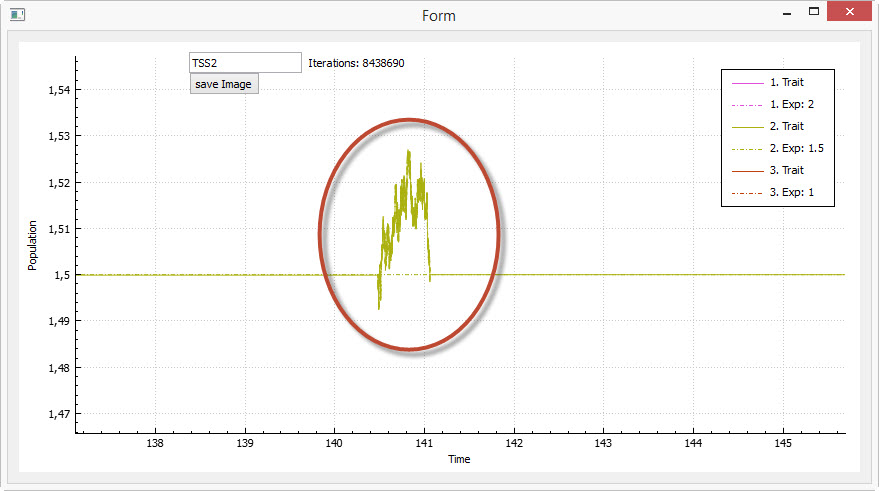
\includegraphics[width=0.8\linewidth]{./TSS_MutationZoom}
				\caption[Invasionsversuch]{Nahaufnahme eines Invasionsversuchs bei dominantem Merkmal}
				\label{fig:TSS_MutationZoom}
			\end{figure}
		\end{frame}	
		\begin{frame}
			\frametitle{Optimierung}
			Näher betrachtete Auswirkungen:
			\begin{figure}[H]
				\centering
				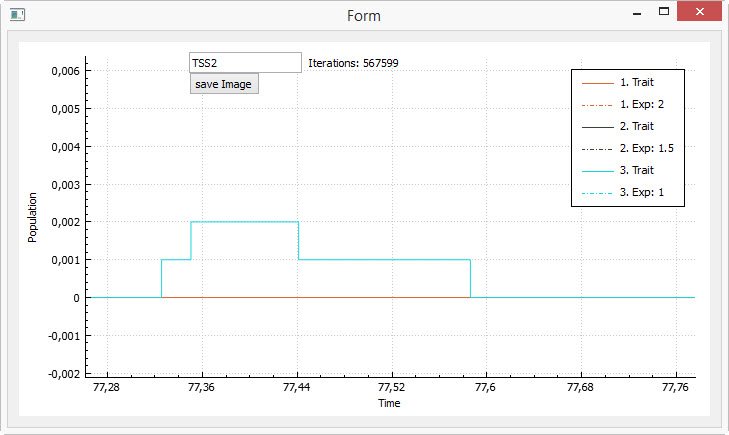
\includegraphics[width=0.8\linewidth]{./TSS_InvasionFail}
				\caption[Invasion Fehlgeschlagen]{Nahaufnahme eines fehlgeschlagenen Invasionsversuchs}
				\label{fig:TSS_InvasionFail}
			\end{figure}
		\end{frame}
		\begin{frame}
			\frametitle{Mutatinospunkte}
			Wie werden die Zeitpunkte für Mutationen bestimmt? \pause
			Mit Raten!
			\begin{itemize}
				\item Geburtsraten der toten Merkmale
				\pause
				\item $ B(x) =  \underbrace{0}_{\text{int. Geb.}} + ( \underbrace{0}_{\text{Mut. von Totem}} + \underbrace{b(y)\cdot n_t(y)}_{\text{Mut. von Dom.}} )\cdot \frac{\mu}{2} $
			\end{itemize}
			Mit dieser Mutationsrate wird eine neue Uhr gestellt die klingelt sobald sich eine Mutation ereignet.
		\end{frame}


\end{document}
% ä Ä ö Ö ü Ü